

\tikzset{every picture/.style={line width=0.75pt}} %set default line width to 0.75pt        

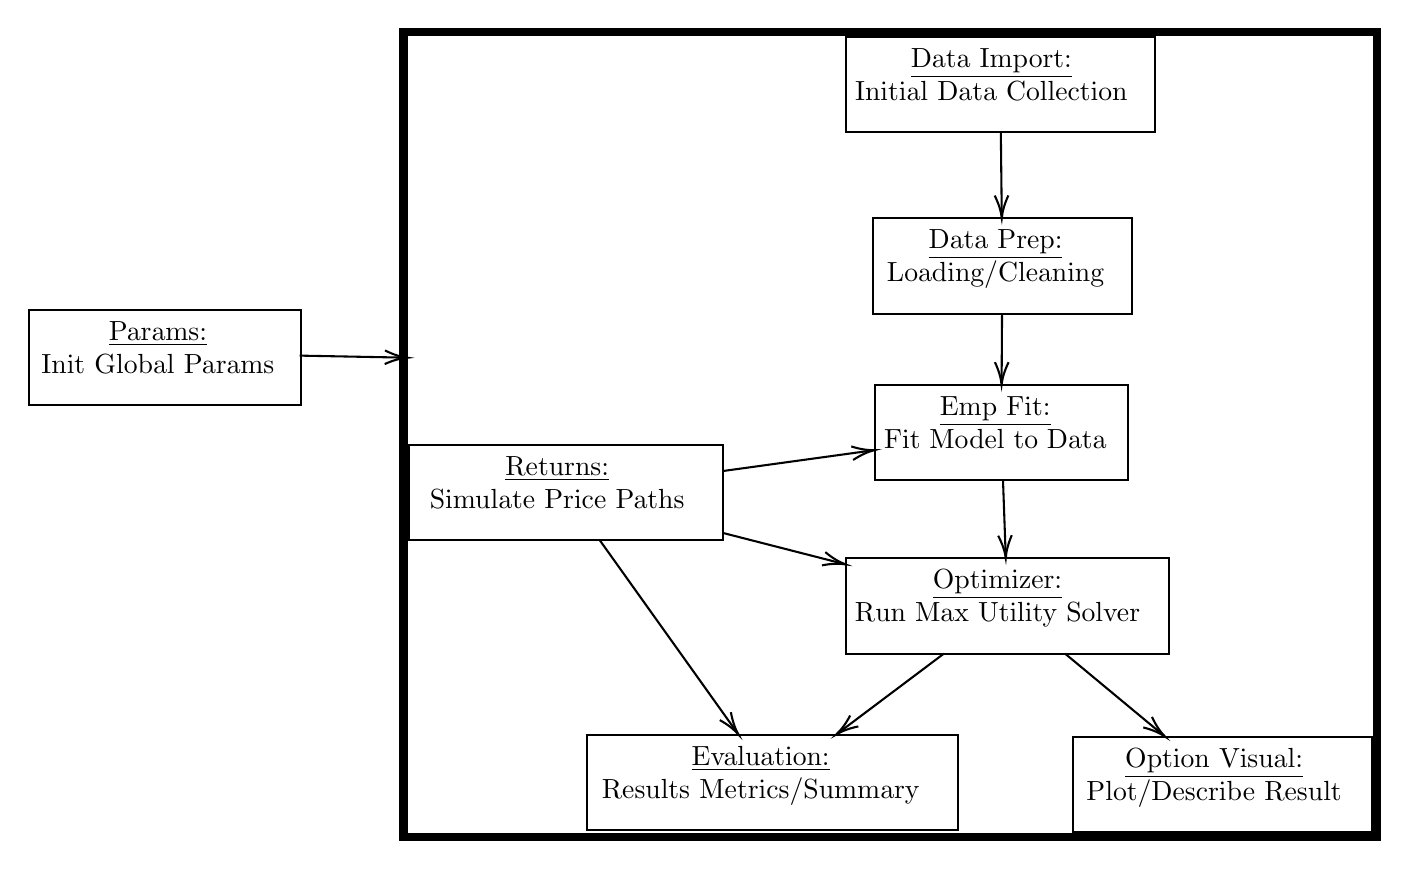
\begin{tikzpicture}[x=0.75pt,y=0.75pt,yscale=-1,xscale=1]
%uncomment if require: \path (0,549); %set diagram left start at 0, and has height of 549

%Shape: Rectangle [id:dp641267805615122] 
\draw  [line width=3]  (192.5,56) -- (661.5,56) -- (661.5,444) -- (192.5,444) -- cycle ;

%Straight Lines [id:da14098325743213436] 
\draw    (142.5,212) -- (192.5,212.96) ;
\draw [shift={(194.5,213)}, rotate = 181.1] [color={rgb, 255:red, 0; green, 0; blue, 0 }  ][line width=0.75]    (10.93,-3.29) .. controls (6.95,-1.4) and (3.31,-0.3) .. (0,0) .. controls (3.31,0.3) and (6.95,1.4) .. (10.93,3.29)   ;

% Text Node
\draw    (12,190) -- (143,190) -- (143,236) -- (12,236) -- cycle  ;
\draw (15,194) node [anchor=north west][inner sep=0.75pt]   [align=left] {\begin{minipage}[lt]{86.63pt}\setlength\topsep{0pt}
\begin{center}
\underline{Params:}\\Init Global Params
\end{center}

\end{minipage}};
% Text Node
\draw  [color={rgb, 255:red, 0; green, 0; blue, 0 }  ,draw opacity=1 ][line width=0.75]   (405.6,58.41) -- (554.6,58.41) -- (554.6,104.41) -- (405.6,104.41) -- cycle  ;
\draw (408.6,62.41) node [anchor=north west][inner sep=0.75pt]   [align=left] {\begin{minipage}[lt]{98.54pt}\setlength\topsep{0pt}
\begin{center}
\underline{Data Import:}\\Initial Data Collection
\end{center}

\end{minipage}};
% Text Node
\draw  [color={rgb, 255:red, 0; green, 0; blue, 0 }  ,draw opacity=1 ][line width=0.75]   (418.59,145.8) -- (543.59,145.8) -- (543.59,191.8) -- (418.59,191.8) -- cycle  ;
\draw (421.59,149.8) node [anchor=north west][inner sep=0.75pt]   [align=left] {\begin{minipage}[lt]{82.12pt}\setlength\topsep{0pt}
\begin{center}
\underline{Data Prep:}\\Loading/Cleaning
\end{center}

\end{minipage}};
% Text Node
\draw  [color={rgb, 255:red, 0; green, 0; blue, 0 }  ,draw opacity=1 ][line width=0.75]   (419.59,226.11) -- (541.59,226.11) -- (541.59,272.11) -- (419.59,272.11) -- cycle  ;
\draw (422.59,230.11) node [anchor=north west][inner sep=0.75pt]   [align=left] {\begin{minipage}[lt]{80.39pt}\setlength\topsep{0pt}
\begin{center}
\underline{Emp Fit:}\\Fit Model to Data
\end{center}

\end{minipage}};
% Text Node
\draw  [color={rgb, 255:red, 0; green, 0; blue, 0 }  ,draw opacity=1 ][line width=0.75]   (280.9,394.59) -- (459.9,394.59) -- (459.9,440.59) -- (280.9,440.59) -- cycle  ;
\draw (283.9,398.59) node [anchor=north west][inner sep=0.75pt]   [align=left] {\begin{minipage}[lt]{118.9pt}\setlength\topsep{0pt}
\begin{center}
\underline{Evaluation:}\\Results Metrics/Summary
\end{center}

\end{minipage}};
% Text Node
\draw  [color={rgb, 255:red, 0; green, 0; blue, 0 }  ,draw opacity=1 ][line width=0.75]   (405.58,309.56) -- (561.58,309.56) -- (561.58,355.56) -- (405.58,355.56) -- cycle  ;
\draw (408.58,313.56) node [anchor=north west][inner sep=0.75pt]   [align=left] {\begin{minipage}[lt]{103.05pt}\setlength\topsep{0pt}
\begin{center}
\underline{Optimizer:}\\Run Max Utility Solver
\end{center}

\end{minipage}};
% Text Node
\draw  [color={rgb, 255:red, 0; green, 0; blue, 0 }  ,draw opacity=1 ][line width=0.75]   (515.2,395.59) -- (659.2,395.59) -- (659.2,441.59) -- (515.2,441.59) -- cycle  ;
\draw (518.2,399.59) node [anchor=north west][inner sep=0.75pt]   [align=left] {\begin{minipage}[lt]{95.13pt}\setlength\topsep{0pt}
\begin{center}
\underline{Option Visual:}\\Plot/Describe Result
\end{center}

\end{minipage}};
% Text Node
\draw  [color={rgb, 255:red, 0; green, 0; blue, 0 }  ,draw opacity=1 ][line width=0.75]   (195.29,255.05) -- (346.29,255.05) -- (346.29,301.05) -- (195.29,301.05) -- cycle  ;
\draw (198.29,259.05) node [anchor=north west][inner sep=0.75pt]   [align=left] {\begin{minipage}[lt]{100.24pt}\setlength\topsep{0pt}
\begin{center}
\underline{Returns:}\\Simulate Price Paths 
\end{center}

\end{minipage}};
% Connection
\draw [color={rgb, 255:red, 0; green, 0; blue, 0 }  ,draw opacity=1 ][line width=0.75]    (480.95,191.8) -- (480.74,224.11) ;
\draw [shift={(480.73,226.11)}, rotate = 270.36] [color={rgb, 255:red, 0; green, 0; blue, 0 }  ,draw opacity=1 ][line width=0.75]    (10.93,-3.29) .. controls (6.95,-1.4) and (3.31,-0.3) .. (0,0) .. controls (3.31,0.3) and (6.95,1.4) .. (10.93,3.29)   ;
% Connection
\draw [color={rgb, 255:red, 0; green, 0; blue, 0 }  ,draw opacity=1 ][line width=0.75]    (481.41,272.11) -- (482.68,307.56) ;
\draw [shift={(482.75,309.56)}, rotate = 267.95] [color={rgb, 255:red, 0; green, 0; blue, 0 }  ,draw opacity=1 ][line width=0.75]    (10.93,-3.29) .. controls (6.95,-1.4) and (3.31,-0.3) .. (0,0) .. controls (3.31,0.3) and (6.95,1.4) .. (10.93,3.29)   ;
% Connection
\draw [color={rgb, 255:red, 0; green, 0; blue, 0 }  ,draw opacity=1 ][line width=0.75]    (346.29,267.63) -- (417.61,257.8) ;
\draw [shift={(419.59,257.52)}, rotate = 532.15] [color={rgb, 255:red, 0; green, 0; blue, 0 }  ,draw opacity=1 ][line width=0.75]    (10.93,-3.29) .. controls (6.95,-1.4) and (3.31,-0.3) .. (0,0) .. controls (3.31,0.3) and (6.95,1.4) .. (10.93,3.29)   ;
% Connection
\draw [color={rgb, 255:red, 0; green, 0; blue, 0 }  ,draw opacity=1 ][line width=0.75]    (346.29,297.39) -- (403.64,312.08) ;
\draw [shift={(405.58,312.58)}, rotate = 194.37] [color={rgb, 255:red, 0; green, 0; blue, 0 }  ,draw opacity=1 ][line width=0.75]    (10.93,-3.29) .. controls (6.95,-1.4) and (3.31,-0.3) .. (0,0) .. controls (3.31,0.3) and (6.95,1.4) .. (10.93,3.29)   ;
% Connection
\draw [color={rgb, 255:red, 0; green, 0; blue, 0 }  ,draw opacity=1 ][line width=0.75]    (452.96,355.56) -- (402.61,393.39) ;
\draw [shift={(401.01,394.59)}, rotate = 323.08000000000004] [color={rgb, 255:red, 0; green, 0; blue, 0 }  ,draw opacity=1 ][line width=0.75]    (10.93,-3.29) .. controls (6.95,-1.4) and (3.31,-0.3) .. (0,0) .. controls (3.31,0.3) and (6.95,1.4) .. (10.93,3.29)   ;
% Connection
\draw [color={rgb, 255:red, 0; green, 0; blue, 0 }  ,draw opacity=1 ][line width=0.75]    (511.28,355.56) -- (557.96,394.31) ;
\draw [shift={(559.5,395.59)}, rotate = 219.7] [color={rgb, 255:red, 0; green, 0; blue, 0 }  ,draw opacity=1 ][line width=0.75]    (10.93,-3.29) .. controls (6.95,-1.4) and (3.31,-0.3) .. (0,0) .. controls (3.31,0.3) and (6.95,1.4) .. (10.93,3.29)   ;
% Connection
\draw [color={rgb, 255:red, 0; green, 0; blue, 0 }  ,draw opacity=1 ][line width=0.75]    (287.21,301.05) -- (352.82,392.96) ;
\draw [shift={(353.98,394.59)}, rotate = 234.48] [color={rgb, 255:red, 0; green, 0; blue, 0 }  ,draw opacity=1 ][line width=0.75]    (10.93,-3.29) .. controls (6.95,-1.4) and (3.31,-0.3) .. (0,0) .. controls (3.31,0.3) and (6.95,1.4) .. (10.93,3.29)   ;
% Connection
\draw [color={rgb, 255:red, 0; green, 0; blue, 0 }  ,draw opacity=1 ][line width=0.75]    (480.36,104.41) -- (480.81,143.8) ;
\draw [shift={(480.83,145.8)}, rotate = 269.35] [color={rgb, 255:red, 0; green, 0; blue, 0 }  ,draw opacity=1 ][line width=0.75]    (10.93,-3.29) .. controls (6.95,-1.4) and (3.31,-0.3) .. (0,0) .. controls (3.31,0.3) and (6.95,1.4) .. (10.93,3.29)   ;

\end{tikzpicture}